\documentclass{standalone}
\usepackage{pgfplots}
\begin{document}
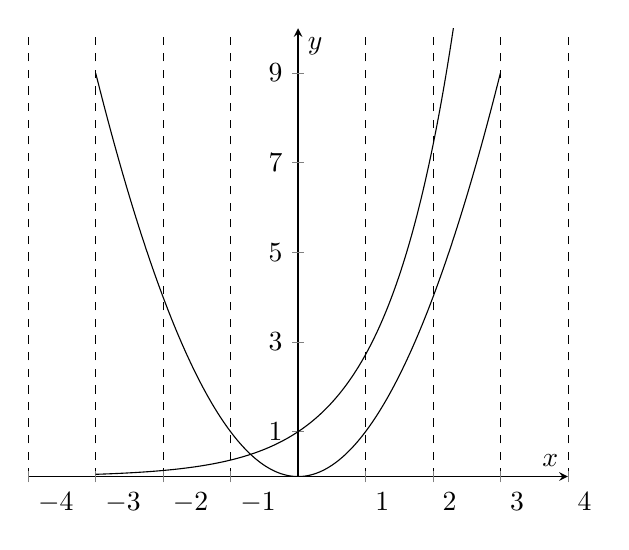
\begin{tikzpicture}
\begin{axis}
[
ymin=0,ymax=10,
xmin=-4,xmax=4,
%clip=false,
xtick=\empty,
ytick=\empty,
extra x ticks={-4, -3, -2, -1, 1, 2, 3, 4},
extra x tick labels={$-4$, $-3$, $-2$, $-1$, $1$, $2$, $3$, $4$},
extra y ticks={1, 3, 5, 7, 9},
extra y tick labels={$1$, $3$, $5$, $7$, $9$},
every extra x tick/.style={
    xticklabel style={anchor=north west},
    grid=major,
    major grid style={very thin,dashed,black}
},
axis lines = center,
xlabel=$x$,ylabel=$y$,
domain=-3:3,
samples=200,
]
\addplot [black] {e^x};
\addplot [black] {x^2};
\node at (axis cs:0.2, -0.28) {$O$} ;
\end{axis}
\end{tikzpicture}
\end{document}
